% ------------------------------------------------------------------------------
% TYPO3 Version 9.1 - What's New - Chapter "Introduction" (German Version)
%
% @author	Michael Schams <schams.net>
% @license	Creative Commons BY-NC-SA 3.0
% @link		http://typo3.org/download/release-notes/whats-new/
% @language	German
% ------------------------------------------------------------------------------
% LTXE-CHAPTER-UID:		7fdf26cc-362160ab-d6c8b905-19722b20
% LTXE-CHAPTER-NAME:	Einführung
% ------------------------------------------------------------------------------

\section{Einführung}
\begin{frame}[fragile]
	\frametitle{Einführung}

	\begin{center}\huge{Einführung}\end{center}
	\begin{center}\huge{\color{typo3darkgrey}\textbf{Die Fakten}}\end{center}

\end{frame}

% ------------------------------------------------------------------------------
% LTXE-SLIDE-START
% LTXE-SLIDE-UID:		207daf88-597d0fcc-15e88d56-22891582
% LTXE-SLIDE-ORIGIN:	db9ce9bf-51fe8c3b-c6a2649f-aa7018b5 English
% LTXE-SLIDE-TITLE:		TYPO3 Version 9.1 - Die Fakten
% ------------------------------------------------------------------------------
\begin{frame}[fragile]
	\frametitle{Einführung}
	\framesubtitle{TYPO3 Version 9.1 - Fakten}

	\begin{itemize}
		\item Veröffentlichungsdatum: 30. Januar 2018
		\item Releasetyp: Sprint Release
	\end{itemize}

	\begin{figure}
		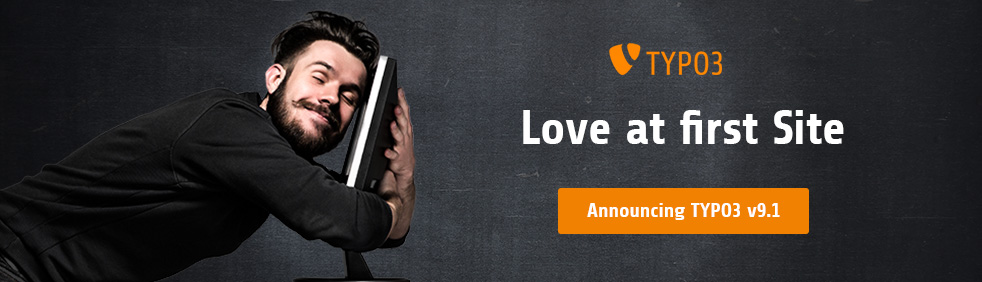
\includegraphics[width=0.95\linewidth]{Introduction/typo3-v91-banner.jpg}
	\end{figure}

\end{frame}

% ------------------------------------------------------------------------------
% LTXE-SLIDE-START
% LTXE-SLIDE-UID:		09e849cf-d075b038-281f93c2-67dfc2db
% LTXE-SLIDE-ORIGIN:		baf0e8fa-b8335fbe-911020ab-489d6156
% LTXE-SLIDE-TITLE:		Systemvoraussetzungen
% ------------------------------------------------------------------------------
\begin{frame}[fragile]
	\frametitle{Einführung}
	\framesubtitle{Systemvoraussetzungen}

	\begin{itemize}
		\item PHP Version 7.2\newline
			\smaller
				(wird möglicherweise für zukünftige Versionen auf PHP 7.1 oder 7.0 herabgesetzt)
			\normalsize

		\item PHP-Einstellungen:

			\begin{itemize}
				\item \texttt{memory\_limit} >= 128M
				\item \texttt{max\_execution\_time} >= 240s
				\item \texttt{max\_input\_vars} >= 1500
				\item Die Compile-Option \texttt{-}\texttt{-disable-ipv6} darf \underline{nicht} verwendet werden
			\end{itemize}

		\item Die meisten von \textbf{Doctrine DBAL} unterstützten Datenbankserver arbeiten auch mit TYPO3.
			Getestete DB-Engines sind zum Beispiel:
	\end{itemize}

	\begin{figure}
		
\includegraphics[width=0.70\linewidth]{Introduction/logo-databases.png}
	\end{figure}

\end{frame}

% ------------------------------------------------------------------------------
% LTXE-SLIDE-START
% LTXE-SLIDE-UID:		6f55946b-665f2825-dc4e0fa8-ea298ea5
% LTXE-SLIDE-ORIGIN:	dfe5c3a8-72a55162-da879770-778ebfec English
% LTXE-SLIDE-TITLE:		Entwicklung, Veröffentlichung und Instandhaltung
% ------------------------------------------------------------------------------
\begin{frame}[fragile]
	\frametitle{Einführung}
	\framesubtitle{Entwicklung, Veröffentlichung und Instandhaltung}

	\textbf{TYPO3 v9}

	\begin{figure}
		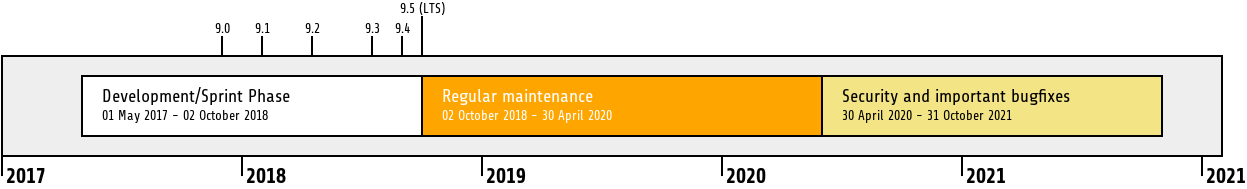
\includegraphics[width=1\linewidth]{Introduction/typo3-v9-lifecycle.png}
	\end{figure}

	\textbf{Erweiterte Unterstützung}\newline
	\smaller
		Die \href{https://typo3.com}{TYPO3 GmbH} bietet weitere Suportmöglichkeiten
		für TYPO3 v9 LTS auch nach dem 31. October 2021 für bis zu zwei weitere Jahre.
	\normalsize

%	\url{https://typo3.com/our-services/extended-support/}

\end{frame}

% ------------------------------------------------------------------------------
% LTXE-SLIDE-START
% LTXE-SLIDE-UID:		2eb41588-b1f9e87a-8f361f3e-e08e5573
% LTXE-SLIDE-ORIGIN:	1c2b096f-e4e0a65c-b0b0d84b-e18889a1 English
% LTXE-SLIDE-TITLE:		TYPO3 v9 Roadmap
% ------------------------------------------------------------------------------
\begin{frame}[fragile]
	\frametitle{Introduction}
	\framesubtitle{TYPO3 v9 Roadmap}

	Voraussichtliche Veröffentlichungen und deren Hauptfokus:

	\begin{itemize}

		\item v9.0 \tabto{1.1cm}12/Dez/2017\tabto{3.4cm}Install Tool und Page Tree Refactoring,\newline
			\tabto{3.4cm}Vereinheitlichte Seitenübersetzungen
		\item
			\begingroup
				\color{typo3orange}
					v9.1 \tabto{1.1cm}30/Jan/2018\tabto{3.4cm}Redirect-Handling
			\endgroup
		\item v9.2 \tabto{1.1cm}10/Apr/2018\tabto{3.4cm}Site Configuration
		\item v9.3 \tabto{1.1cm}12/Jun/2018\tabto{3.4cm}URL Routing
		\item v9.4 \tabto{1.1cm}04/Sep/2018\tabto{3.4cm}Frontend Editing
		\item v9.5 \tabto{1.1cm}02/Okt/2018\tabto{3.4cm}LTS Release

	\end{itemize}

	\smaller
		\url{https://typo3.org/news/article/typo3-v9-roadmap/}
	\normalsize

\end{frame}

% ------------------------------------------------------------------------------
% LTXE-SLIDE-START
% LTXE-SLIDE-UID:		cea4f2db-80fd5ac7-e1a83104-c9754ae3
% LTXE-SLIDE-ORIGIN:	27b13d1c-5c952e3e-d4422d93-0a8a273d English
% LTXE-SLIDE-TITLE:		Installation
% ------------------------------------------------------------------------------
\begin{frame}[fragile]
	\frametitle{Einführung}
	\framesubtitle{Installation}

	\begin{itemize}
		\item Empfohlene \textit{klassische} Installationsschritte unter Linux/Mac OS X\newline
			(DocumentRoot ist beispielsweise \texttt{/var/www/site/htdocs}):
		\begin{lstlisting}
			$ cd /var/www/site
			$ wget --content-disposition get.typo3.org/9.1
			$ tar xzf typo3_src-9.1.0.tar.gz
			$ cd htdocs
			$ ln -s ../typo3_src-9.1.0 typo3_src
			$ ln -s typo3_src/index.php
			$ ln -s typo3_src/typo3
			$ touch FIRST_INSTALL
		\end{lstlisting}

		\item Symbolische Links unter Microsoft Windows:

			\begin{itemize}
				\item unter Windows XP/2000 kann \texttt{junction} benutzt werden
				\item unter Windows Vista und Windows 7 oder höher kann \texttt{mklink} benutzt werden
			\end{itemize}

	\end{itemize}
\end{frame}

% ------------------------------------------------------------------------------
% LTXE-SLIDE-START
% LTXE-SLIDE-UID:		09998aca-7e523ecb-d92605dd-20fb3450
% LTXE-SLIDE-ORIGIN:	2991c08b-8831f59c-56bc188c-e05b8e92 English
% LTXE-SLIDE-TITLE:		Installation mit Composer
% ------------------------------------------------------------------------------
\begin{frame}[fragile]
	\frametitle{Installation und Upgrade}
	\framesubtitle{Installation mit \texttt{composer}}

	\begin{itemize}
		\item Installation mit \textit{composer} unter Linux/Mac OS X

			\begin{lstlisting}
				$ cd /var/www/site/
				$ composer create-project typo3/minimal
			\end{lstlisting}

		\item Alternativ kann man eine benutzerdefinierte \texttt{composer.json} Datei erstellen und ausführen:

			\begin{lstlisting}
				$ composer install
			\end{lstlisting}

			Ein Beispielsdatei \texttt{composer.json} kann heruntergeladen werden unter:\newline
			\small
				\href{https://git.typo3.org/TYPO3CMS/Distributions/Base.git/blob/HEAD:/composer.json}{git.typo3.org/TYPO3CMS/Distributions/Base.git/blob/HEAD:/composer.json}
			\normalsize

	\end{itemize}
\end{frame}

% ------------------------------------------------------------------------------
% LTXE-SLIDE-START
% LTXE-SLIDE-UID:		c1d4ec33-f1b72470-0b0d3733-ae08e0b3
% LTXE-SLIDE-ORIGIN:	3bc1e21e-cf2c23c4-b1d641af-8e351b92 English
% LTXE-SLIDE-TITLE:		Upgrade zu TYPO3 Version 9
% ------------------------------------------------------------------------------
%\begin{frame}[fragile]
%	\frametitle{Introduction}
%	\framesubtitle{Upgrade to TYPO3 Version 9.x}
%
%	\begin{itemize}
%		\item Upgrades sind nur möglich von TYPO3 v8 LTS
%		\item TYPO3 < v8 LTS sollten zunächst auf TYPO3 v8 LTS aktualisiert werden
%	\end{itemize}
%
%	\begin{itemize}
%
%		\item Upgrade-Anleitung:\newline
%			\smaller\url{https://wiki.typo3.org/Upgrade#Upgrading_to_9.1}\normalsize
%		\item Offizielles TYPO3 Guide "TYPO3 Installation and Upgrading":
%			\smaller\url{https://docs.typo3.org/typo3cms/InstallationGuide}\normalsize
%		\item Generelles Vorgehen:
%			\begin{itemize}
%				\item Prüfen, ob Mindestvoraussetzungen erfüllt sind \small(PHP, MySQL, etc.)
%				\item Das \textbf{deprecation\_*.log} der TYPO3 Instanz durchsehen
%				\item Alle Extensions auf den aktuellsten Stand bringen
%				\item Neuen TYPO3 Quellcode entpacken und im Install Tool den Upgrade Wizard ausführen
%				\item Das Startmodul für BE Benutzer prüfen (optional)
%			\end{itemize}
%	\end{itemize}
%
%\end{frame}
%
% ------------------------------------------------------------------------------
